\documentclass[12pt, a4paper, Spanish]{article}
\usepackage[utf8]{inputenc}
\usepackage{
    graphicx,
    enumitem,
    chngcntr,
    csquotes,
    amsmath,
    mathptmx,
    amssymb,
    float,
    amssymb,
    amsfonts,
    fullpage,
    caption
}
\usepackage{hyperref}
\usepackage{xcolor}
\hypersetup{colorlinks=true, linkcolor=black, urlcolor=cyan, citecolor=black}
\graphicspath{{imagenes/}}

\begin{document}


\begin{figure}[H]
    \centering
    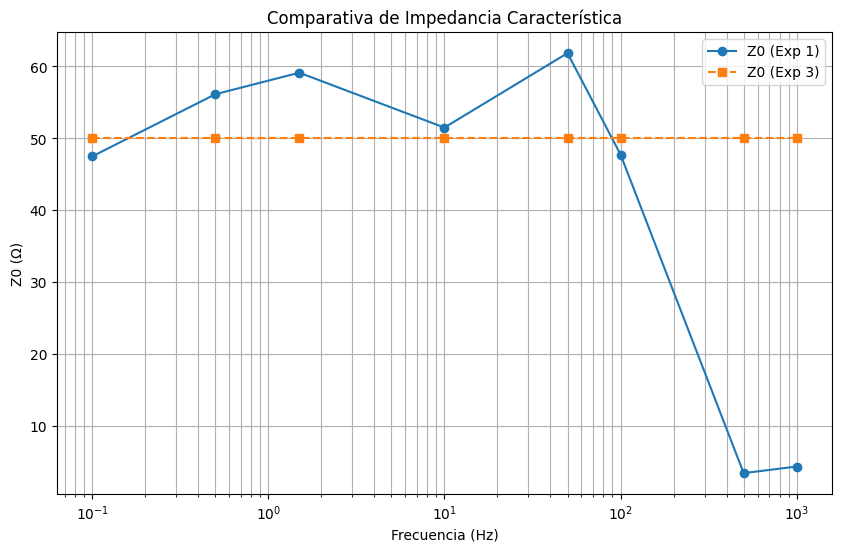
\includegraphics[width=0.7\textwidth]{impedancia-caracteristica-atenuador-simple.png}
    \caption{Impedancia característica del atenuador simple.}
    \label{fig:impedancia_simple}
\end{figure}

\begin{figure}[H]
    \centering
    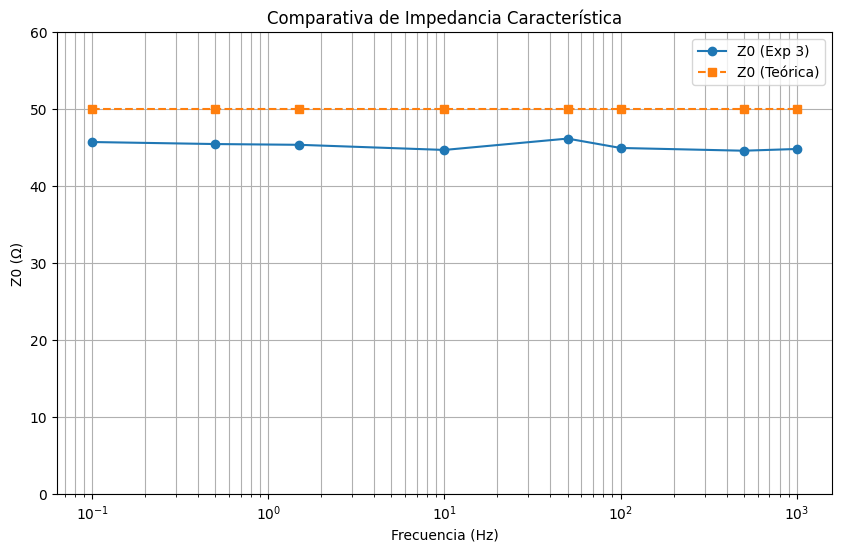
\includegraphics[width=0.7\textwidth]{impedancia-caracteristica-atenuador-en-cascada.png}
    \caption{Impedancia característica del atenuador en cascada.}
    \label{fig:impedancia_cascada}
\end{figure}


\begin{figure}[H]
    \centering
    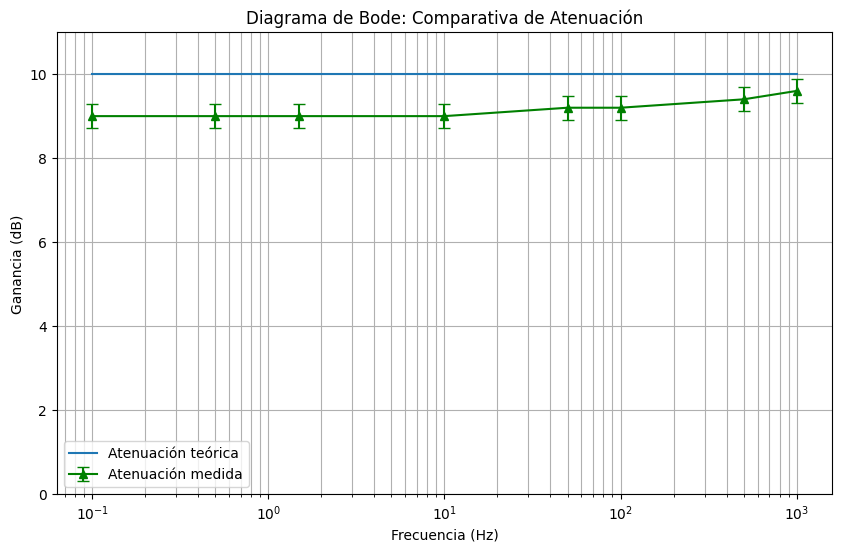
\includegraphics[width=0.7\textwidth]{atenuacion-atenuador-simple.png}
    \caption{Atenuación del atenuador simple.}
    \label{fig:atenuacion_simple}
\end{figure}

\begin{figure}[H]
    \centering
    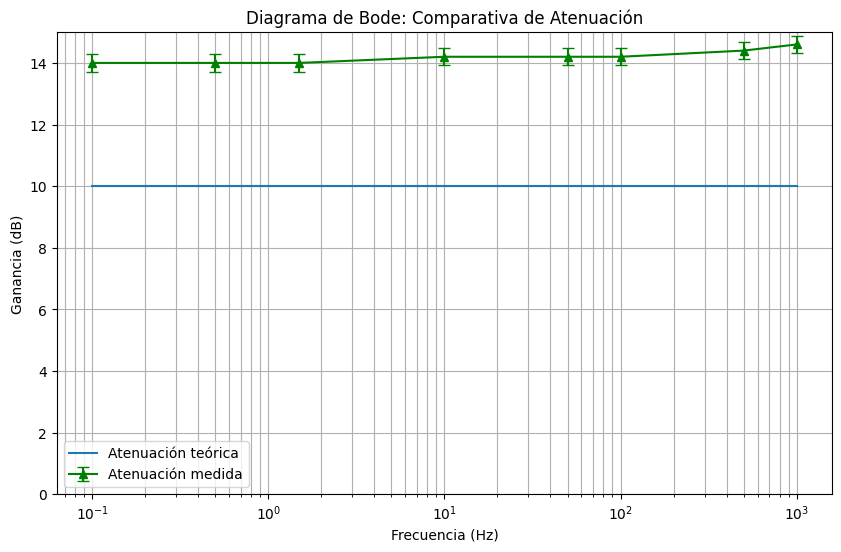
\includegraphics[width=0.7\textwidth]{atenuacion-atenuador-en-cascada.png}
    \caption{Atenuación del atenuador en cascada.}
    \label{fig:atenuacion_cascada}
\end{figure}

\end{document}
